
  \documentclass[a4paper,titlepage,12pt]{article}
  \usepackage[english]{babel}
  \usepackage{longtable}
  \usepackage{hyperref}
  \usepackage{multirow}
  \usepackage{lscape}
  \usepackage[top=2cm,bottom=2cm,left=1cm,right=1cm]{geometry}
  \usepackage{float}
  \usepackage[utf8]{inputenc}
  \usepackage[pdftex]{epsfig}  
  \DeclareGraphicsRule{.pdftex}{pdf}{.pdftex}{}  
  \title{Report}
  
  
  \begin{document}
  \maketitle
  \tableofcontents
  \listoftables
  \listoffigures
  \newpage
  \section{Tables}    
    \begin{longtable}{lccccc}\caption{Summary descriptives table by groups of `DROPOUT'}\\
    \hline  
     & Completed high school & Dropped out of high school & \multirow{2}{*}{       OR       } & \multirow{2}{*}{p.ratio} & \multirow{2}{*}{p.overall}\\ 
 &         N=226         &            N=24            &                  &         &           \\ 
  
    \hline
    \hline     
    \endfirsthead 
    \multicolumn{6}{l}{\tablename\ \thetable{} \textit{-- continued from previous page}}\\ 
    \hline
     & Completed high school & Dropped out of high school & \multirow{2}{*}{       OR       } & \multirow{2}{*}{p.ratio} & \multirow{2}{*}{p.overall}\\ 
 &         N=226         &            N=24            &                  &         &           \\ 

    \hline
    \hline  
    \endhead   
    \hline
    \multicolumn{6}{l}{\textit{continued on next page}} \\ 
    \endfoot   
    \multicolumn{6}{l}{}  \\ 
    \endlastfoot 
    SOCPROB: &                       &                            &                  &         &   0.038  \\ 
$\qquad$Yes 9th grade social problems &      210 (92.9\%)      &         19 (79.2\%)         &       Ref.       &  Ref.   &          \\ 
$\qquad$No 9th grade social problems &      16 (7.08\%)       &         5 (20.8\%)          & 3.48 [1.02;10.2] &  0.046  &          \\ 
REPEAT: &                       &                            &                  &         &   0.001  \\ 
$\qquad$Didn't repeat a grade &      199 (88.1\%)      &         14 (58.3\%)         &       Ref.       &  Ref.   &          \\ 
$\qquad$Repeated a grade &      27 (11.9\%)       &         10 (41.7\%)         & 5.23 [2.05;13.0] &  0.001  &          \\ 
ADDSC &      51.0 (11.7)      &        59.2 (9.60)         & 1.07 [1.03;1.11] &  0.001  &  $<$0.001   \\ 
 
    \hline
    \end{longtable}
  \newpage
      
    \begin{longtable}{lcccccc}\caption{Available data by groups of `DROPOUT'}\\
    \hline  
     & [ALL] & Completed high school & Dropped out of high school &      method       & select & Fact OR/HR \\ 
 
    \hline 
    \hline  
    \endfirsthead 
    \multicolumn{7}{l}{\tablename\ \thetable{} \textit{-- continued from previous page}}\\ 
    \hline
     & [ALL] & Completed high school & Dropped out of high school &      method       & select & Fact OR/HR \\ 
 
    \hline
    \hline 
    \endhead   
    \hline
    \multicolumn{7}{l}{\textit{continued on next page}} \\ 
    \endfoot    
    \multicolumn{7}{l}{}  \\ 
    \endlastfoot 
    SOCPROB &  250  &          226          &             24             &    categorical    &  ALL   &     --    \\ 
REPEAT &  250  &          226          &             24             &    categorical    &  ALL   &     --    \\ 
ADDSC &  250  &          226          &             24             & continuous-normal &  ALL   &     1      \\ 

    \hline
    \end{longtable}
  \section{Figures}
  \subsection{univariate}
  
  \begin{figure}[H]
  \begin{center}
  \caption{ADDSC}
  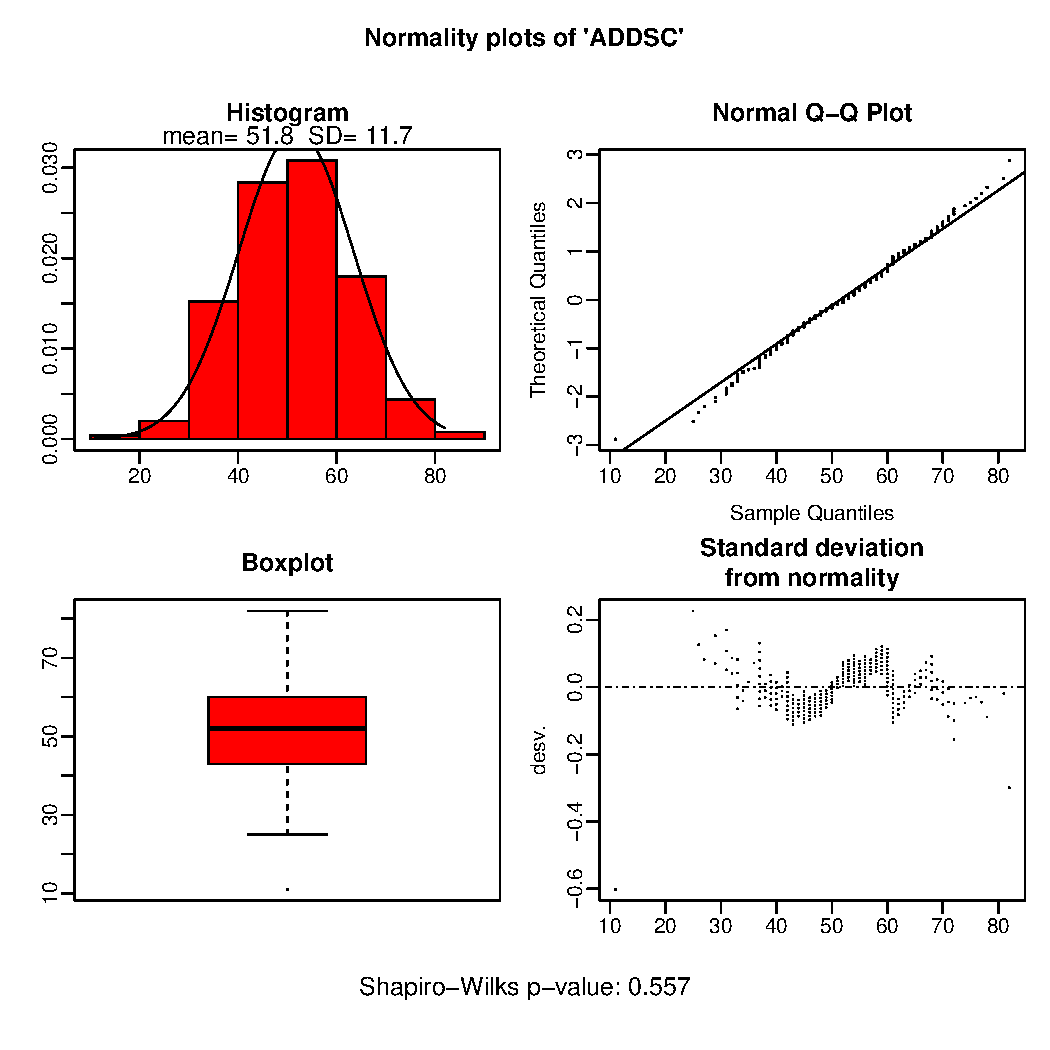
\includegraphics[width=17cm]{./allgroups_report_figures/uni_ADDSC.pdf}
  \end{center}
  \end{figure}
  
  \begin{figure}[H]
  \begin{center}
  \caption{REPEAT}
  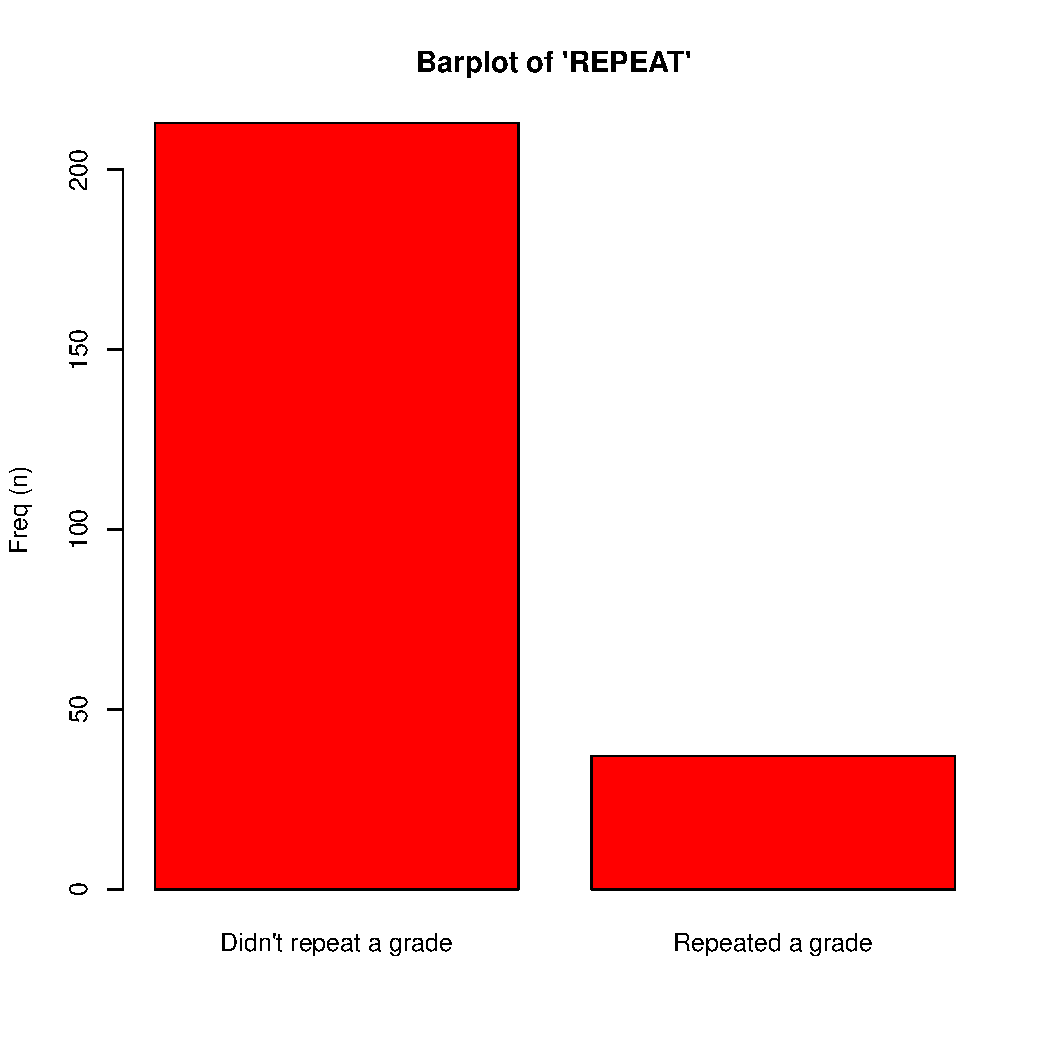
\includegraphics[width=17cm]{./allgroups_report_figures/uni_REPEAT.pdf}
  \end{center}
  \end{figure}
  
  \begin{figure}[H]
  \begin{center}
  \caption{SOCPROB}
  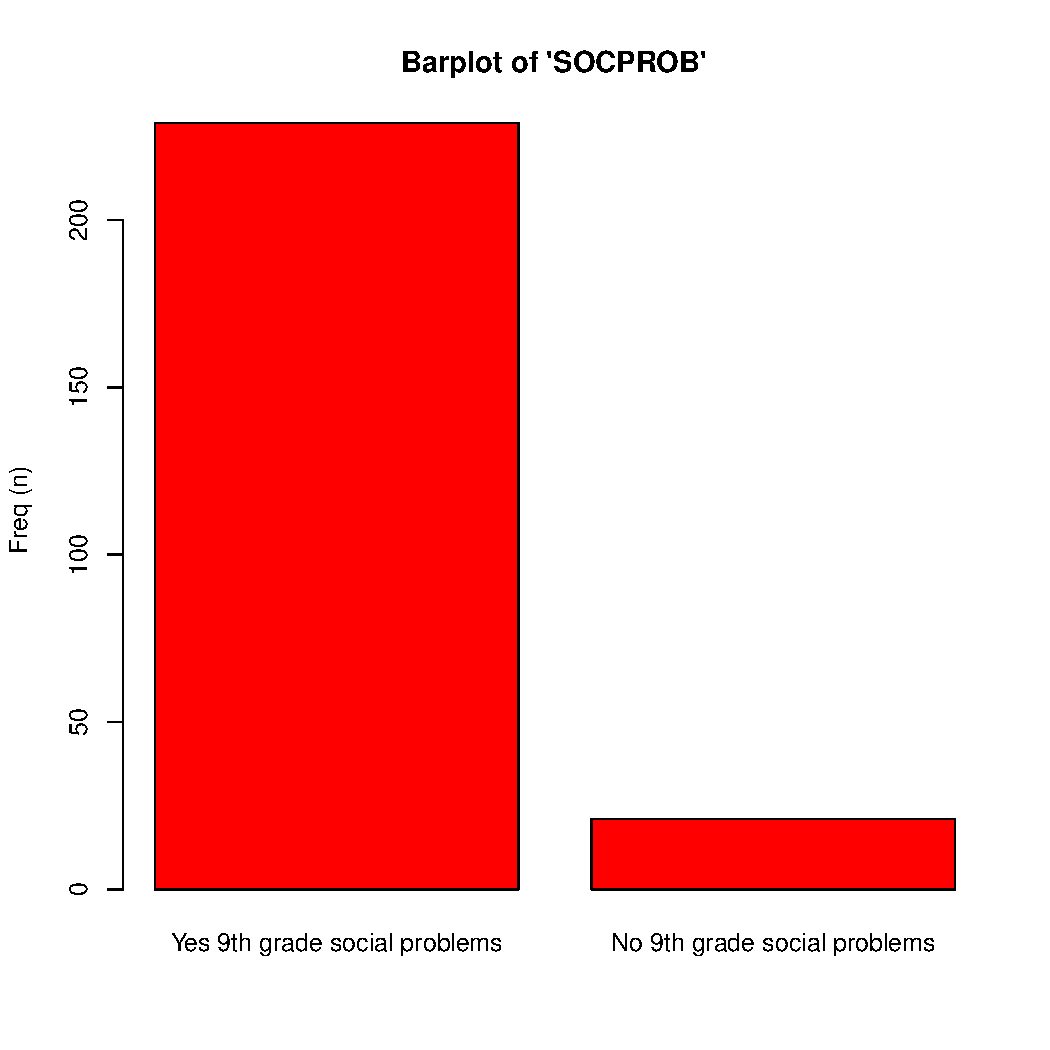
\includegraphics[width=17cm]{./allgroups_report_figures/uni_SOCPROB.pdf}
  \end{center}
  \end{figure}
  \subsection{bivariate}
    \begin{figure}[H]
    \begin{center}
    \caption{ADDSC}
    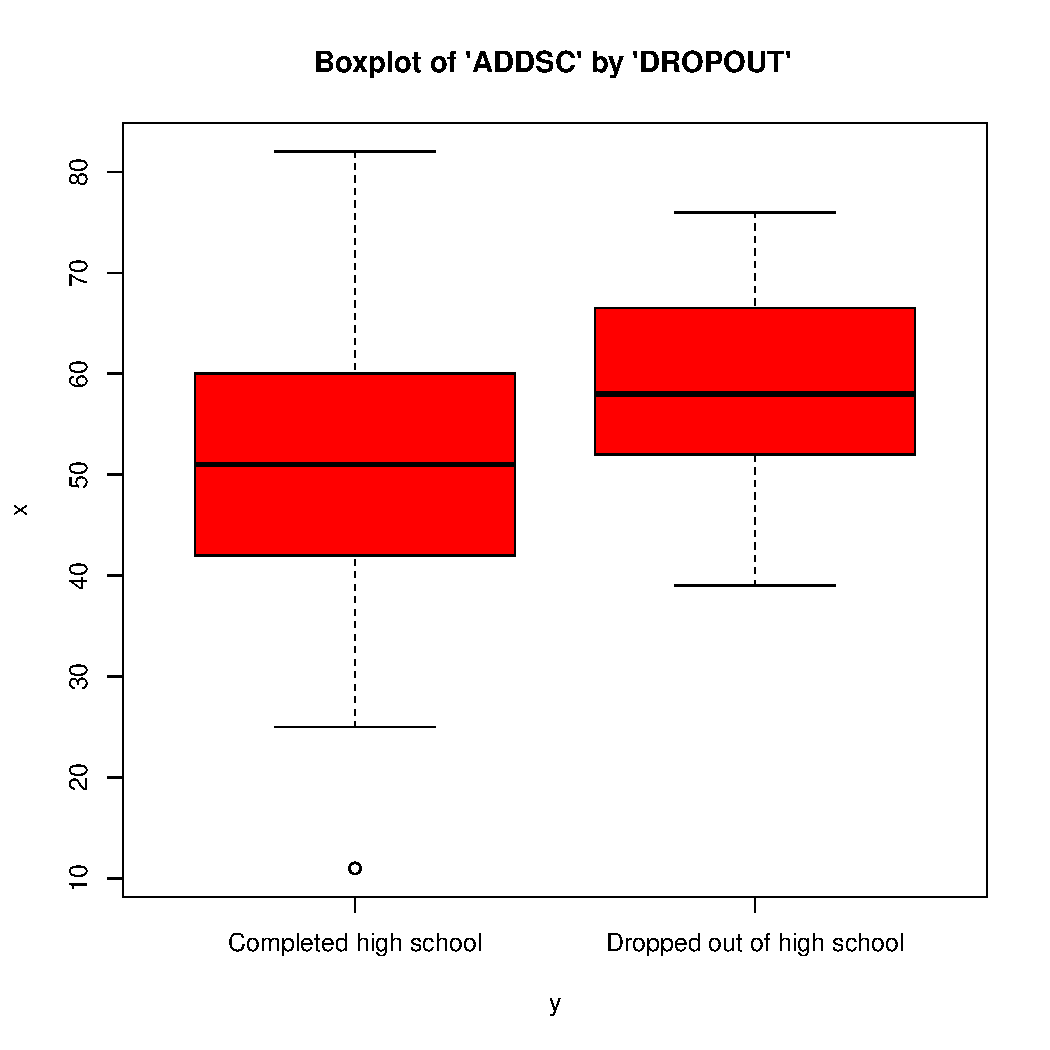
\includegraphics[width=17cm]{./allgroups_report_figures/bivar_ADDSC.pdf}
    \end{center}
    \end{figure}
    
    \begin{figure}[H]
    \begin{center}
    \caption{REPEAT}
    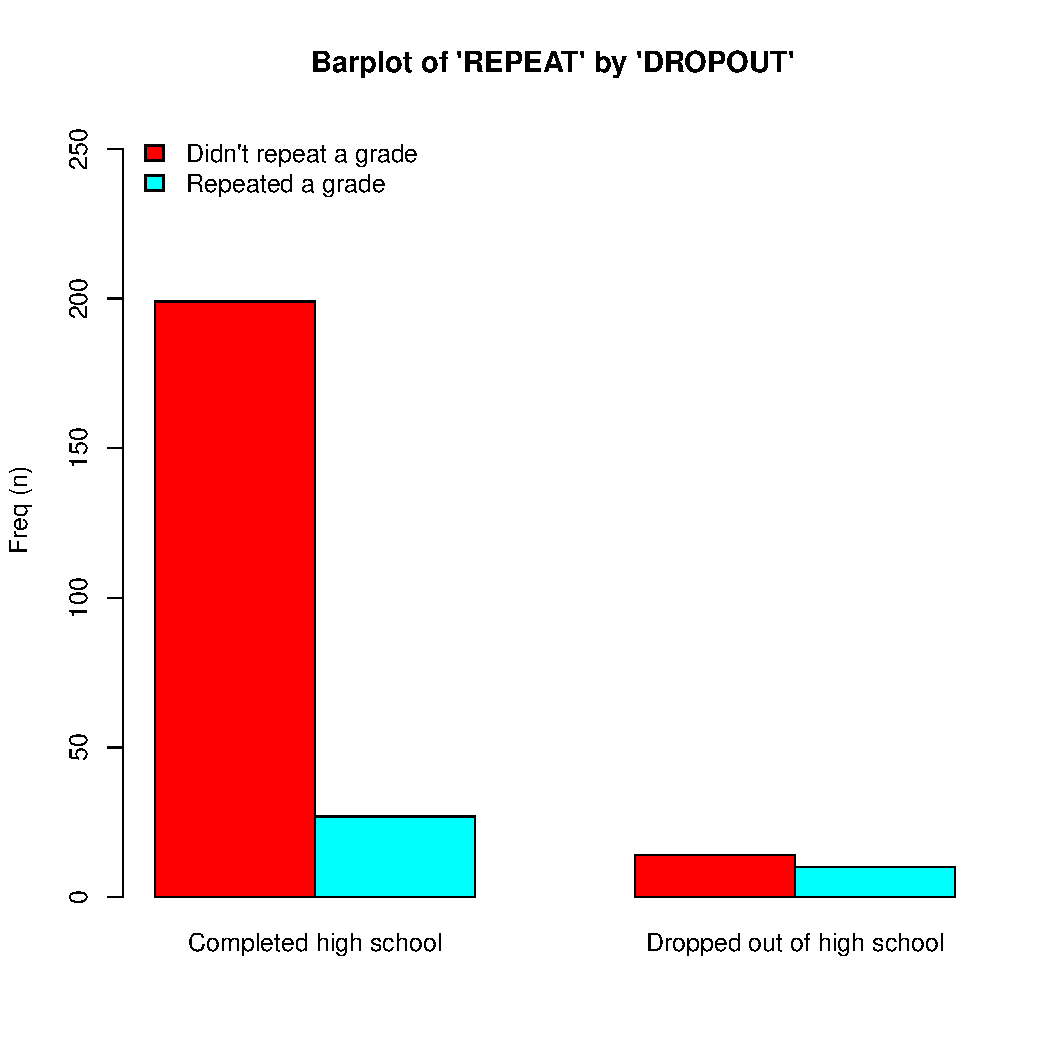
\includegraphics[width=17cm]{./allgroups_report_figures/bivar_REPEAT.pdf}
    \end{center}
    \end{figure}
    
    \begin{figure}[H]
    \begin{center}
    \caption{SOCPROB}
    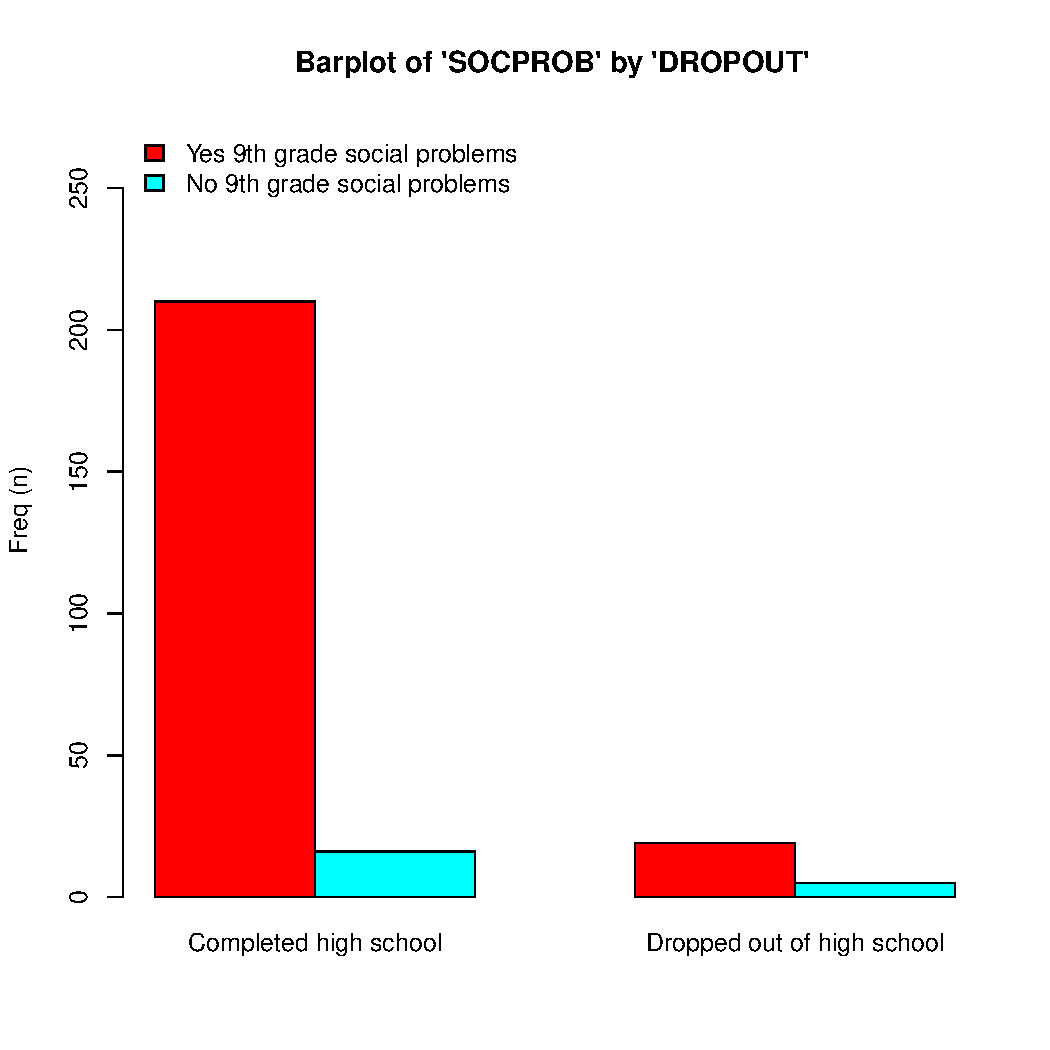
\includegraphics[width=17cm]{./allgroups_report_figures/bivar_SOCPROB.pdf}
    \end{center}
    \end{figure}
    
  \end{document}
  
